% Draft 2026-10-20. Numbers marked \pending{} await runs in progress.
\documentclass{article}
\usepackage{spconf,amsmath,amssymb,graphicx,booktabs}
\usepackage[T1]{fontenc}
\usepackage{times}
\usepackage{microtype}
\usepackage{xcolor}
\usepackage[hidelinks]{hyperref}
\newcommand{\pending}[1]{\textcolor{red}{[#1]}}
\title{Recovery Lives in $u$, Conditioning Acts in $r$:\\
Where Arbitrary-Scale Super-Resolution Gains Come From}
\name{Anonymous authors}
\address{Draft for internal review}
\begin{document}
\maketitle

\begin{abstract}
Arbitrary-scale super-resolution (ASISR) networks pair an image encoder with an implicit decoder that also receives the target pixel size (cell). Decoder and cell designs have multiplied, yet their gains shrink at large scales. We explain this with two frequency coordinates. Measured per band, recovery is a function of frequency normalised by the low-resolution Nyquist limit, $u$. It is the same for four decoder designs on a shared encoder (within 0.01). Training and a stronger encoder raise it only for $u\ge 1$. The cell, in contrast, acts on the output as a low-pass in high-resolution frequency $r$. For large mismatch, its cost is predicted by the recovered energy at the frequencies it attenuates. Because a fixed $r$ moves to larger $u$ as scale grows, where little is recovered, the cell's leverage vanishes. Doubling the cell costs 2.1--2.5\,dB at $\times2$, 0.13\,dB at $\times4$ and at most 0.03\,dB at $\times6$. All tests were pre-registered with frozen predictions; failed predictions are reported. The account predicts that capacity spent on the decoder or the cell is wasted at large scales, and we verify this with matched training \pending{D1--D3, T1--T3 final}.
\end{abstract}
\begin{keywords}
Arbitrary-scale super-resolution, implicit neural representation, frequency analysis, scale conditioning
\end{keywords}

\section{Introduction}
LIIF~\cite{chen2021liif} reconstructs an image at continuous coordinates. It decodes local encoder features together with the query offset and the target cell size. Many decoders followed: LTE's local Fourier estimator~\cite{lee2022lte}, integrated positional encoding~\cite{liu2021ipe}, attention-based decoders~\cite{cao2023ciaosr}, neural operators~\cite{wei2023srno}, Gaussian splatting~\cite{hu2024gaussiansr} and filtered heat fields~\cite{becker2025thera}. A recent benchmark finds that gains from decoder design are small and saturate~\cite{nasir2026empirical}. Frequency analyses describe low-pass behaviour~\cite{fsds2024}, probe responses~\cite{kawai2026frequency} or scale anchoring~\cite{wang2026scaleanchoring}. They do not say \emph{where} a decoder or the cell can still change the output, or why that space disappears as the scale grows.

We answer with two coordinates. For scale $s$ and HR frequency $r$ (cycles per HR pixel), let $u=2sr$ be the frequency relative to the LR Nyquist limit. Our claims are:
\begin{enumerate}
\item \textbf{Recovery lives in $u$.} Per-band recovery $R(u)$ is nearly scale-independent and decoder-independent. Training and the encoder change it only above $u\approx0.75$.
\item \textbf{Conditioning acts in $r$.} Changing the cell multiplies the native output by an approximately scale-independent low-pass $w(r)$. Its cost is bounded by the recovered energy at those $r$, so the cell's leverage decays with scale.
\item \textbf{Consequence.} At large scales, decoder capacity and cell input matter little, while encoder capacity still matters. We test this with matched training.
\end{enumerate}
That cell inputs can occasionally hurt is already known~\cite{liu2021ipe}. Our contribution is a quantitative account of where any decoder- or cell-side change can act at all. Every experiment followed a frozen protocol (code, predictions and scoring hashed before results); Table~\ref{tab:gates} lists outcomes, including failures.

\section{Setup}
\textbf{Models.} LIIF, LTE and SC-INR (an LTE-derived variant whose cell enters through an analytic sinc weight) share an EDSR-baseline encoder~\cite{lim2017edsr} and the LIIF training recipe (DIV2K~\cite{agustsson2017div2k}, scales $\mathcal U(1,4)$, 1000 epochs, three seeds). We add GaussianSR~\cite{hu2024gaussiansr} (EDSR-baseline encoder) and RDN-BTC~\cite{zhang2018rdn,pak2023btc}. For matched comparisons we train LIIF for 200 epochs with an identical recipe and EDSR-baseline, RDN or SwinIR~\cite{liang2021swinir} encoders, a reduced decoder ($2\times64$ MLP) or no cell input.

\textbf{Data and degradation.} Fresh DIV2K valid 0869--0900 (never used in this project), Set14~\cite{zeyde2010single}, BSD100~\cite{martin2001database} and Urban100~\cite{huang2015urban}. We take centre $240^2$ crops and bicubic anti-aliased downsampling at $\times\{2,3,4,6\}$; $\times6$ lies outside training support.

\textbf{Measurements.} After a 4-pixel shave, errors are split by Chebyshev FFT radius into $u$-bins of width $0.25$. Then $R(u)=1-\mathrm{MSE}_u/E_u$, with $E_u$ the target energy in the bin. The cell sweep multiplies the native cell by $m\in[\tfrac12,2]$ (11 values).

\section{Recovery lives in $u$}
Fig.~\ref{fig:rec}a shows $R(u)$ for four scales. Below the LR Nyquist limit ($u<1$) networks and bicubic interpolation both recover most energy. Between $u=0.75$ and $2$ the network recovers far more: at $u=1$, $0.68$ versus $0.20$ for bicubic; at $u=1.5$, $0.36$ versus $0.04$. Curves at different scales nearly coincide, but only approximately. Our frozen tolerance (spread $\le0.05$) held in 45/54 cases; the misses sit in the $\times2$ bin closest to the HR Nyquist limit.

\emph{Decoders do not move $R(u)$.} On a shared EDSR-baseline encoder, LIIF, LTE, SC-INR and GaussianSR differ by at most $0.010$ in every bin (18/18 and 18/18; Fig.~\ref{fig:rec}b). Correspondingly, their PSNR differs by only $0.03$--$0.06$\,dB, shrinking from $\times2$ to $\times6$.

\emph{Training and the encoder do.} Between epoch 100 and 1000, $R(u)$ rises by up to $0.045$ for $u\ge1$ (12/12 bins). It is unchanged below $u<0.75$ ($\le0.008$; 9/9; Fig.~\ref{fig:rec}c). With decoder and recipe fixed, an RDN encoder raises $R(u)$ only for $u\ge1$ \pending{T1/T2 final; epoch-50 interim: 12/12 and 9/9}. External checkpoints (RDN-BTC, official EDSR) underperformed under our degradation and are not used as encoder evidence.

\begin{figure*}[t]\centering
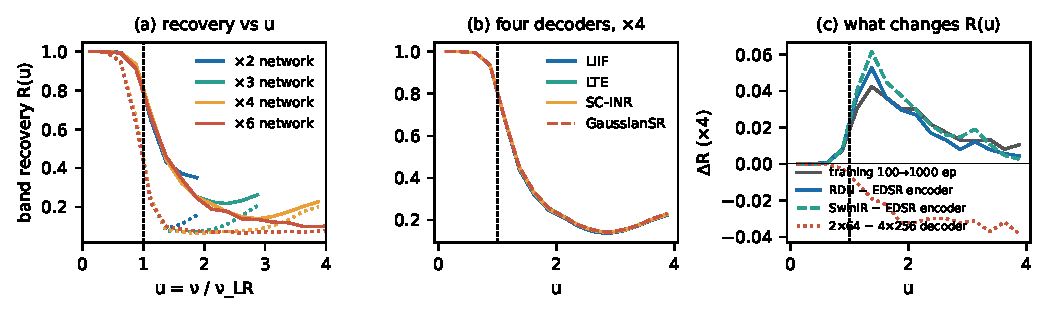
\includegraphics[width=\textwidth]{figures/fig1_recovery.pdf}
\vspace{-6mm}
\caption{(a) Band recovery $R(u)$ at four scales (solid: mean of three decoders and three seeds; dotted: bicubic). (b) Four decoders on the same encoder. (c) Change in $R(u)$ from further training and from a stronger encoder.}
\label{fig:rec}
\end{figure*}

\section{Conditioning acts in $r$}
Let $P_1$ be the native output and $P_m$ the output with cell multiplied by $m$. Projected per band, we find
\begin{equation}
P_{m,b}\approx w_{m}(r_b)\,P_{1,b},\quad w_m(r)\in\mathbb R,
\label{eq:filter}
\end{equation}
a low-pass in HR frequency whose shape barely depends on scale (Fig.~\ref{fig:cell}a). Writing $e_b=T_b-P_{1,b}$ for the native error, Eq.~\eqref{eq:filter} gives the exact expansion
\begin{equation}
\Delta\mathrm{MSE}_b=2(1-w)\,\mathrm{Re}\langle e_b,P_{1,b}\rangle+(1-w)^2\|P_{1,b}\|^2 .
\label{eq:leverage}
\end{equation}
If the native cell is calibrated, the first-order term is small. The cost is then governed by $(1-w)^2\|P_{1,b}\|^2$: the energy the network actually emits at the frequencies the cell attenuates. At fixed $r$, larger scales place that energy at larger $u$, where little has been recovered. This is why the cell's leverage decays with scale.

\emph{Tests.} For $m=2$, the cost peaks at $r\approx0.25$ for every model, seed and scale (36/36; Fig.~\ref{fig:cell}b). Its magnitude tracks recovered energy (Spearman $0.77$--$0.78$). The second-order term ranks per-band cost with $\rho=0.86$--$0.91$ and accounts for $70$--$77\%$ of it. Cost decays monotonically with scale for all nine model--seed pairs (Fig.~\ref{fig:cell}c), and also for GaussianSR and RDN-BTC. The native cell is close to calibrated: the best fixed multiplier improves on it by at most $0.017$\,dB. Its optimum drifts slightly above $m=1$ at $\times4$--$\times6$, so the frozen ``native is optimal'' gate failed (20/27).

\emph{Limits of the model.} For small mismatch ($m=4/3$) the first-order term dominates and Eq.~\eqref{eq:filter} does not predict cost. The peak at $r\approx0.25$ holds only for the LIIF family; GaussianSR and BTC peak elsewhere. We had also predicted that a too-small cell (requesting detail) would cost more than a too-large one, by analogy with prior-mismatch asymmetry. The opposite held (33/144), so we withdraw that hypothesis.

\begin{figure*}[t]\centering
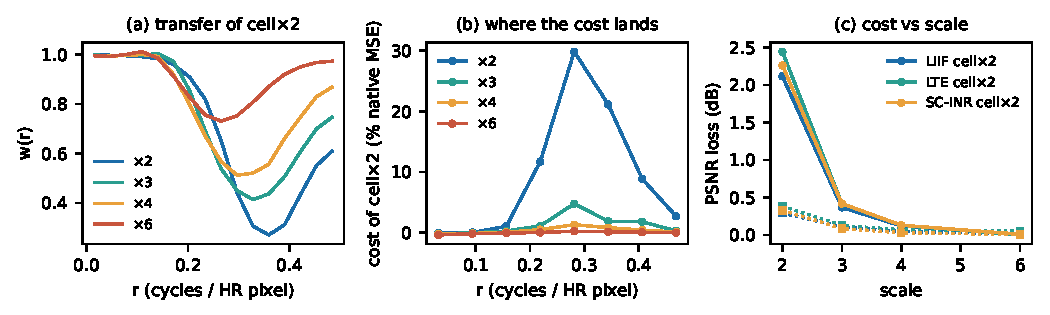
\includegraphics[width=\textwidth]{figures/fig2_cell.pdf}
\vspace{-6mm}
\caption{(a) Spectral transfer $w(r)$ of doubling the cell (LTE, Set14). (b) Where its cost lands in HR frequency. (c) PSNR cost of doubling (solid) or halving (dotted) the cell, by scale.}
\label{fig:cell}
\end{figure*}

\section{Consequence: where to spend capacity}
\begin{table}[t]\centering\small
\caption{Matched 200-epoch LIIF training, PSNR change (dB) relative to the EDSR-baseline LIIF, non-DC, DIV2K 0869--0900.}
\label{tab:budget}
\begin{tabular}{lcccc}\toprule
Arm & $\times2$ & $\times3$ & $\times4$ & $\times6$\\\midrule
decoder $2\times64$ & \pending{} & \pending{} & \pending{} & \pending{}\\
no cell input & \pending{} & \pending{} & \pending{} & \pending{}\\
RDN encoder & \pending{} & \pending{} & \pending{} & \pending{}\\
SwinIR encoder (ep.\,50) & \pending{} & \pending{} & \pending{} & \pending{}\\\bottomrule
\end{tabular}
\end{table}
The two-coordinate account makes a design prediction, frozen before training. Shrinking the decoder or removing the cell should cost little at $\times4$ and above, while a stronger encoder should still help (Table~\ref{tab:budget}) \pending{results}.

\begin{table}[t]\centering\small
\caption{Pre-registered predictions and outcomes.}
\label{tab:gates}
\begin{tabular}{p{5.3cm}r}\toprule
Prediction & Outcome\\\midrule
$R(u)$ spread across scales $\le0.05$ & 45/54 \textbf{fail}\\
decoders within 0.03 (four decoders) & 18/18, 18/18\\
training raises only $u\ge1$ & 12/12; 9/9\\
cell$\times2$ cost peaks at $r\in[0.19,0.375)$ & 36/36 (LIIF family)\\
cost $\sim$ recovered energy ($\rho\ge0.7$) & 0.77--0.78\\
leverage decays with scale & 9/9\\
native cell optimal & 20/27 \textbf{fail}\\
too-small cell costs more & 33/144 \textbf{fail}\\
$\ge$80\% of cost at $u\ge1$ & 75\% \textbf{fail}\\
RDN raises only $u\ge1$ & \pending{}\\
decoder budget D1--D3 & \pending{}\\\bottomrule
\end{tabular}
\end{table}

\section{Limitations and conclusion}
We study bicubic degradation, centre crops, convolutional and Transformer encoders and LIIF-style training. The $u$-collapse is approximate. The filter model of the cell holds for large mismatch only. Its frequency locus is specific to decoder families. Within these limits, ASISR gains lie in what the encoder learns above the LR Nyquist limit. The cell is an HR-frequency control whose reach is set by that recovery. Decoder and cell innovations should therefore be evaluated where $u\lesssim2$ at the scale of interest, and capacity at large scales belongs in the encoder.

\bibliographystyle{IEEEbib}
\bibliography{refs}
\end{document}
